\section{Preliminaries}\label{sec:prelims}
In this section we introduce the definitions, lemmas, and tools that we will use
throughout the work, providing the details that are needed in later sections.

\subsection{Itemsets mining}\label{sec:itemdef}
Given a ground set $\Itm$ of \emph{items}, let $\prob$ be a probability
distribution on $2^{\Itm}$. A \emph{transaction} $\tau\subseteq\Itm$ is a single
sample drawn from $\prob$. The \emph{length} $|\tau|$ of a transaction $\tau$ is
the number of items in $\tau$.   We
call a subset of $\Itm$ an \emph{itemset}. For any itemset $A$, let
$T(A)=\{\tau\subseteq\Itm ~:~ A\subseteq \tau\}$ be the \emph{support set} of
$A$. The members of the set $T(A)$ are all the transactions built on $\Itm$
that contain the itemset $A$. We define the \emph{true frequency} $\tfreq(A)$ of
$A$ with respect to $\prob$ as the probability that a transaction sampled from
$\prob$ contains $A$:
\[
\tfreq(A) = \sum_{\tau\in T(A)}\prob(\tau)\enspace.
\]

A \emph{dataset} $\Ds$ is a bag of $n$
transactions $\Ds=\{\tau_1,\dots,\tau_n ~:~ \tau_i\subseteq\Itm\}$, i.e., of $n$
\emph{independent identically distributed} (i.i.d.) samples from $\prob$.
Given a (observed) dataset $\Ds$, let $T_\Ds(A)$ denote the set of
transactions in $\Ds$ containing $A$. The \emph{frequency} of $A$ in $\Ds$ is
the fraction of transactions in $\Ds$ that contain $A$: $f_\Ds(A)=
|T_\Ds(A)|/|\Ds|$. It is easy to see that $f_\Ds(A)$ is the \emph{empirical
average} (and an \emph{unbiased estimator}) for $\tfreq(A)$: ${\mathbf
E}[f_\Ds(A)]=\tfreq(A)$.

Traditionally, the interest has been on extracting the set of \emph{Frequent
Itemsets} (FIs) from $\Ds$ with respect to a minimum frequency threshold
$\theta\in(0,1]$~\citep{AgrawalIS93}, that is, the set
\[
\FI(\Ds,\Itm,\theta)=\{A\subseteq\Itm ~:~ f_\Ds(A)\ge\theta\}\enspace.\]

In most applications the final goal of data mining is to gain a better
understanding of the \emph{process generating the data}, i.e., of the
distribution $\prob$, through the true frequencies $\tfreq$, which are
\emph{unknown} and only approximately reflected in the dataset $\Ds$. Therefore,
in this work, we are interested in finding the itemsets with \emph{true}
frequency $\tfreq$ at least $\theta$ for some $\theta\in(0,1]$. We call these
itemsets the \emph{True Frequent Itemsets} (TFIs) and denote their set as
\[
\TFI(\prob,\Itm,\theta)=\{A\subseteq\Itm ~:~ \tfreq(A)\ge\theta\}\enspace.\]

If one is only given a \emph{finite} number of random samples (the dataset
$\Ds$) from $\prob$, as it is usually the case, one can not aim at finding the
exact set $\TFI(\prob,\Itm,\theta)$: no assumption can be made on the
set-inclusion relationship between $\TFI(\prob,\Itm,\theta)$ and
$\FI(\Ds,\Itm,\theta)$, because an itemset $A\in\TFI(\prob,\Itm,\theta)$ may not
appear in $\FI(\Ds,\Itm,\theta)$, and vice versa. One can instead try to
\emph{approximate} the set of TFIs. This is the focus of this work.

\paragraph{Goal.} Given an user-specified
parameter $\delta\in(0,1)$, we aim at providing a threshold
$\hat{\theta}\ge\theta$ such that $\mathcal{C}=\FI(\Ds,\Itm,\hat{\theta})$
\emph{well approximates} $\TFI(\prob,\Itm,\theta)$, in the sense that
\begin{enumerate*}
  \item With probability at least $1-\delta$, $\mathcal{C}$ does not contain any
    false positive:
  \[
  \Pr(\exists A\in\mathcal{C} ~:~ \tfreq(A)<\theta)<\delta\enspace.\]
\item $\mathcal{C}$ contains as many TFIs as possible.

  \end{enumerate*}
The method we present does not make \emph{any} assumption about $\prob$. It uses
information from $\Ds$, and retrieves a large fraction of the TFIs, guaranteeing 
that, with probability at least $1-\delta$, no false positive is included.

\subsection{Vapnik-Chervonenkis dimension}\label{sec:prelvcdim}
Let $D$ be a domain and $\range$ be a collection of subsets from $D$. We call $\range$ a
\emph{range set on $D$}. The Vapnik-Chernovenkis (VC) Dimension of $\range$ is
a measure of its complexity or expressiveness~\cite{VapnikC71}. A finite bound
on the VC-dimension implies a bound on the number of random samples
required for approximate the relative sizes of the subsets in $\range$. We
outline here some basic definitions and results and refer the reader to the
works of~\citet[Chap.~3]{MohriRT12}, \citet[Sect.~3]{BoucheronBL05},
and~\citet{Vapnik99} for more details on VC-dimension. See
Sect.~\ref{sec:prevworkvc} for applications of VC-dimension in computer science.

Given $B\subseteq D$, the \emph{projection of $\range$ on $B$} is the set
$P_\range(B)=\{ B\cap A ~:~ A\in\range\}$. We say that the set $B$ is
\emph{shattered} by $\range$ if $P_\range(B)=2^B$.

\begin{definition}\label{def:empvcdim}
  Given a set $B\subseteq D$, the \emph{empirical Vapnik-Chervonenkis
  (VC) dimension of $\range$ on $B$}, denoted as $\EVC(\range,B)$ is
  the cardinality of the largest subset of $B$ that is shattered by
  $\range$. The \emph{VC-dimension of $\range$} is defined as $\VC(\range)=\EVC(\range,D)$.
\end{definition}

Note that an arbitrary large range set $\range$ defined on an arbitrary large
domain $D$ can have a bounded VC-dimension. A simple
example is the family of intervals in $[0,1]$ (i.e. $D$ is all the points in
$[0,1]$ and $\range$ all the intervals $[a,b]$, such that $0\leq a\leq b\leq 1$). Let
$A=\{x,y,z\}$ be the set of three points $0<x<y<z<1$. No interval in $\range$ can
define the subset $\{x,z\}$ so the VC-dimension of this range set is less than
3~\cite[Lemma 10.3.1]{Matousek02}. Another example is shown in
Fig.~\ref{fig:rectangles}.
\begin{figure}[ht]
  \centering
  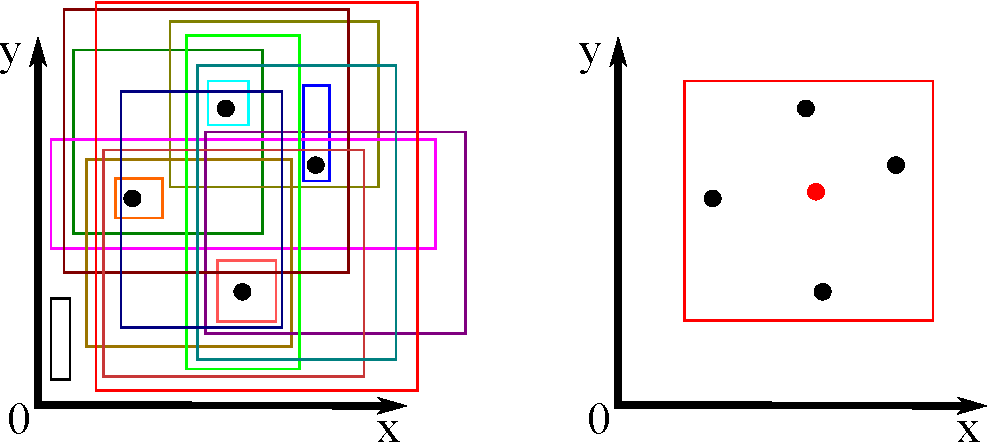
\includegraphics[width=.7\textwidth,keepaspectratio]{rectangles}
  \caption{Example of range set and VC-dimension. The domain is the
  plane $\mathbb{R}^2$ and the range set is the set of all
  \emph{axis-aligned rectangles}. The figure on the left shows graphically that
  it is possible to shatter a set of four points using 16 rectangles. On the
  right instead, one can see that it is impossible to shatter five points, as,
  for any choice of the five points, there will always be one (the red point in
  the figure) that is internal to the convex hull of the other four, so it would
  be impossible to find an axis-aligned rectangle containing the four points
  but not the internal one. Hence $\VC(\range)=4$.
  \fabio{[Need to change figure and/or caption?]}
  }
  \label{fig:rectangles}
\end{figure}

Given a probability distribution $\nu$ on the elements of $D$, the main
application of (empirical) VC-dimension in statistics and learning theory is in
computing the number of samples needed to approximate the probabilities
associated to the ranges through their empirical averages.  Formally, let
$X_1^k=(X_1,\dotsc,X_k)$ be a collection of independent identically distributed
random variables taking values in $D$, sampled according to $\nu$.
For a set $A\subseteq D$, let $\nu(A)$ be the probability that a sample from
$\nu$ belongs to the set $A$, and let
\[
\nu_{X_1^k}(A)=\frac{1}{k}\sum_{j=1}^k\mathds{1}_A(X_j),\]
where $\mathds{1}_A$ is the indicator function for $A$. The function
$\nu_{X_1^k}(A)$ is the \emph{empirical average} of $\nu(A)$ on $X_1^k$.

\begin{definition}\label{def:eapprox}
  Let $\range$ be a range set on a domain
  $D$ and $\nu$ be a probability distribution on $D$. For $\varepsilon\in(0,1)$,
  an \emph{$\varepsilon$-approximation to $(\range,\nu)$} is a bag $S$ of
  elements of $D$ such that
  \[
  \sup_{A\in\range}|\nu(A)-\nu_S(A)|\le\varepsilon\enspace.\]
\end{definition}

Given a sample $S$ of $\ell$ points of $D$ sampled according to the distribution
$\nu$, and a parameter $\delta\in(0,1)$, an upper bound to the empirical
VC-dimension of $\range$ on $S$ allows to compute an $\varepsilon$ such that $S$
is an $\varepsilon$-approximation to $(\range,\nu)$ with probability at least
$1-\delta$, as stated in the following result.

\begin{theorem}\label{thm:eapproxempir}
	Let $\range$ be a range set on a domain $D$ and let $\nu$ be a distribution
	on $D$. Let $S$ be a collection of $\ell$ elements from $D$ sampled
	independently according to $\nu$, and let $\EVC(\range,S)\le d$. Given
	$\delta\in(0,1)$, let
	\begin{equation}\label{eq:evceapprox}
		\varepsilon = 2c\max_{r\in\range}\sqrt{|r\cap S|}\frac{\sqrt{2d}}{\ell} +
		\sqrt{\frac{2\ln\frac{4}{\delta}}{\ell}}\enspace.
	\end{equation}
	Then $S$ is a $\varepsilon$-approximation for $(\range,\nu)$ with
	probability at least $1-\delta$.
\end{theorem}
This theorem follows from known results in statistical learning theory, as shown
in the Appendix.
%We present the proof of this theorem in the Appendix.

% THE FOLLOWING IS HOW STUFF WAS BEFORE PRESENTING THE NEW BOUND
%An $\varepsilon$-approximation can be constructed by sampling a sufficient
%number of points of $D$ according to the distribution $\nu$, provided an upper
%bound to the VC-dimension of $\range$ or to its empirical VC-dimension is known:
%
%\begin{theorem}[Thm.~2.12~\citep{HarPS11}%, see also~\citep{LiLS01}
%]\label{thm:eapprox}
%  Let $\range$ be a range set on a domain
%  $D$ with $\VC(\range)\le d$, and let $\nu$ be a distribution on $D$. Given
%  $\delta\in(0,1)$ and a positive integer $\ell$, let
%  \begin{equation}\label{eq:vceapprox}
%    \varepsilon = \sqrt{\frac{c}{\ell}\left(d + \ln\frac{1}{\delta}\right)}
%  \end{equation}
%  where $c$ is an universal positive constant. Then, a bag of $\ell$
%  elements of $D$ sampled \emph{independently} according to $\nu$ is an
%  $\varepsilon$-approximation to $(\range,\nu)$ with probability at least
%  $1-\delta$.
%\end{theorem}
%The constant $c$ is at most $0.5$~\citep{LofflerP09}.

%The following theorem bounds the maximum deviation $\varepsilon$ in terms of
%the empirical VC-dimension and of other sample-dependent quantities. We present
%its proof in the Appendix.
%
%\begin{theorem}\label{thm:eapproxempir}
%	Let $\range$ be a range set on a domain $D$ and let $\nu$ be a distribution
%	on $D$. Let $S$ be a collection of $\ell$ elements from $D$ sampled
%	independently according to $\nu$, and let $\EVC(\range,S)\le d$. Given
%	$\delta\in(0,1)$, let
%	\begin{equation}\label{eq:evceapprox}
%		\varepsilon = 2\max_{r\in\range}\sqrt{|r\cap
%		S|}\frac{\sqrt{2\min\left\{\ln|\range|,d\ln\frac{en}{d}\right\}}}{\ell} +
%		\sqrt{\frac{2\ln\frac{4}{\delta}}{\ell}}\enspace.
%	\end{equation}
%	Then $S$ is a $\varepsilon$-approximation for $(\range,\nu)$ with
%	probability at least $1-\delta$.
%\end{theorem}

\subsection{Antichains}\label{sec:antichains}
In our algorithm we make a heavy use of \emph{antichains}.

\begin{definition}\label{def:antichain}
	Let $D$ be a domain and $\mathcal{S}$ be a collection of subsets of $D$:
	$\mathcal{S}\subseteq 2^D$. An \emph{antichain} on $\mathcal{S}$ is a subset
	$\mathcal{A}$ of $\mathcal{S}$ such that for any two elements $A' \neq A''$ of
	$\mathcal{A}$ we have neither $A'\subseteq A''$ nor $A''\subseteq A'$.

	A \emph{maximal antichain} is an antichain that is not a proper subset of
	any other antichain.
\end{definition}

\begin{fact}\label{fact:largestantichain}
	The largest antichain on $\mathcal{S}$ is a maximal antichain.
\end{fact}

Computing the size of the largest antichain on a collection $\mathcal{S}$ is
equivalent to finding the maximum matching in a bipartite graph: if $m$ is the
size of the maximum matching (i.e., the number of matched pairs of vertices),
then the largest antichain has size $|\mathcal{S}|-m$~\citep{FordF62}. The graph
contains two nodes (one on each side) for each element of $\mathcal{S}$. There
is an edge between a node $v$ on the l.h.s.~and a node $u$ on the r.h.s.~iff the
element of $\mathcal{S}$ corresponding to $v$ is a \emph{proper} subset of the
element of $\mathcal{S}$ corresponding to $u$. Computing a maximum matching on
in this bipartite graph can be done in polynomial time in the size of
$\mathcal{S}$ (more precisely in time $O(\sqrt{|\mathcal{S}|}|E|)$, where $|E|$
is the number of edges in the graph)~\citep{HopcroftK73}.

% THE FOLLOWING IS VERY OLD STUFF THAT WE MOST PROBABLE WILL NOT NEED.
%\subsection{Statistical hypothesis testing}\label{sec:stat_tests}
%We develop our methods to identify the True Frequent Itemsets within the
%framework of \emph{statistical
%hypothesis testing}. In statistical hypothesis testing, one uses some data
%$Y$ to evaluate a \emph{null hypothesis} $H$, whose rejection corresponds to claiming
%the identification of a significant phenomenon. A \emph{test statistic} $t_H(Y)$ associated
%to the hypothesis is computed from the data. If the $t_H(Y)$ belongs to a predefined
%\emph{acceptance region} (a subset of the domain of $t_H$), then $H$ is
%accepted, otherwise it is rejected. The acceptance region is defined a priori
%in such a way that the probability of a \emph{false positive}, i.e., the
%probability of accepting a true null hypothesis (corresponding to a non significant
%phenomenon), is at most some \emph{critical
%value} $\alpha$. Accepting a true null hypothesis is also called a ``Type-1
%error''. Often, defining an acceptance region as function of $\alpha$ is done
%implicitly, and instead of verifying whether the statistics belongs to it, one
%evaluates the associated \emph{$p$-value}, that is, the probability that the
%statistic $t_H$ is at least as extreme as the value observed on the given data,
%conditioning on the null hypothesis being true, and reject $H$ if the $p$-value
%is not larger than $\alpha$. Another important factor for a
%statistical test is its \emph{power}, that is the probability that the test
%correctly rejects the null hypothesis when the null hypothesis is false (also
%defined as $1-\Pr[\text{Type-2 error}]$, where a ``Type-2 error'' consists in
%non rejecting a false null hypothesis).
%
%In our scenario, the na\"{i}ve method to employ statistical hypothesis testing
%to find the TFIs is to define a null hypothesis $H_A$ for every itemset $A$,
%with $H_A =$ ``$\tfreq(A) < \theta$'', and to compute the $p$-value for such null
%hypothesis using $f_\Ds (A)$ as statistic. In particular, the $p$-value is given
%by the probability that the frequency of $A$ in a random dataset (with the same
%number of transactions of $\Ds$) sampled from $\prob$ is $\ge f_\Ds (A)$
%\emph{conditioning} on the event ``$\tfreq(A)< \theta$''. This is easy to
%compute given that the number of transactions in a dataset that contain $A$ has
%a Binomial distribution whose parameters are the size of the dataset and the
%true frequency of $A$ (\emph{Binomial test}). If the $p$-value is ``small enough'', the
%null hypothesis is rejected, that is $A$ is flagged as a TFI. The issue, in
%our case, is that we are considering a number of itemsets, that is we are facing a
%\emph{multiple hypothesis testing} problem~\cite{LiuZW11}. In this case, one is
%interested in controlling the probability of false discoveries among all the
%hypotheses tested, i.e., in controlling the \emph{Family-Wide Error Rate}.
%
%\begin{definition}\label{def:FWER}
%  The Family-Wise Error Rate (FWER) of a statistical test is the probability of reporting
%  at least one false discovery.
%\end{definition}
%
%In order to achieve the desired FWER, one must define a sequence of critical
%values for the individual hypotheses, that is, implicitly define a sequence of
%acceptance region for the test statistics. The \emph{Bonferroni
%correction}~\citep{DudoitSB03} is a widely-employed method to define such a
%sequence. In its simplest form, the Bonferroni correction suggests to compare
%the $p$-value of each hypothesis to the critical value $\alpha/m$, where $\alpha$ is the
%desired FWER, and $m$ is the number of hypotheses to be tested.  The Bonferroni
%correction is not a good choice to identify TFIs,
%%as it is known to be
%l%oose when the hypotheses are correlated, which is indeed the case
%fo%r TFIs.  Moreover,
%since the statistical power of methods that use the Bonferroni
%correction decreases with the number of hypotheses tested. In practical cases
%there would be hundreds or thousands of TFIs, making the use of the Bonferroni
%correction impractical if one wants to achieve high statistical power.

%If we were to use the same critical
%value $\alpha$ as in the single case, we could potentially produce a number
%of spurious discoveries~\cite{LiuZW11}. In order to avoid this issue, a multiple
%hypothesis correction is employed, like the Bonferroni
%correction~\citep{DudoitSB03} %(see Section~\ref{sec:statpow}).

%When only one hypothesis is considered,
%the null hypothesis is rejected when the $p$-value is at most $\alpha$, with
%$\alpha$ usually set to $0.05$ or $0.01$. This guarantees that the
%\emph{significance level}, that is the probability of incorrectly flagging an
%itemset as True Frequent (Type-1 error), is bounded by $\alpha$.

%In our scenario, since we are considering a number of itemsets, we are facing a
%\emph{multiple hypothesis testing} problem. If we were to use the same
%procedure as the single hypothesis case, we could potentially produce a number
%of spurious discoveries~\cite{LiuZW11}. In order to avoid this issue, a multiple
%hypothesis correction is employed, like the Bonferroni
%correction~\citep{DudoitSB03} %(see Section~\ref{sec:statpow}).

%\begin{definition}\label{def:FWER}
%  The Family-Wise Error Rate (FWER) of a statistical test is the probability that at
%  least one false positive is reported as significant.
%\end{definition}

%The Bonferroni correction guarantees that the FWER is bounded by $\alpha$.  A
%recently proposed alternative to  bound the FWER is to bound the False Discovery
%Rate (FDR), that in our case correspond to the proportion of false discoveries
%among the TFI. The use of the FDR allows to produce in output a larger number of
%patterns, since a small proportion of false discoveries are tolerated in the output;
%however, in frequent itemset mining mining the number of patterns produced is usually high,
%therefore having a smaller number of high quality discoveries is preferable to
%reporting a larger number of patterns containing some false discoveries.

%\iffalse
%\begin{definition}\label{def:FDR}
% The False Discovery Rate~\citep{BenjaminiH95} (FDR) is the expected proportion of
% false positives among all itemsets that are reported as significant.
%\end{definition}
%\fi

%We focus in this work on identifying a highly reliable collections of high
%quality itemsets, and therefore aim to identify True Frequent Itemsets while
%bounding the FWER of our method, that is we bound the probability that the
%collection of itemsets reported by our method contains \emph{any} spurious
%discovery (any itemeset that is not True Frequent)
%
%Another important factor for a statistical test is its \emph{power}, that is the
%probability that the test correctly rejects the null hypothesis when the null
%hypothesis is false (also defined as $1-\Pr[\text{Type-2 error}]$).
